\section{Automatisierte Entscheidungsfindung}

Die ganzheitliche Planung von Landwirtschaftsbetrieben ist ein komplexes Problem das makroskopische sowie mikroskopische Faktoren einbeziehen muss. Ein sehr früher Ansatz um alle Umwelteinflüsse zu bewerten und die Ergebnisse in einer Optimierung der Prozesse infließen zu lassen, ist das \textit{Life Cycle Assessment}, kurz LCA. Dabei werden alle Einflüsse in den Lebenszyklusphasen des Produkts bzw. Services identifiziert. Das Ergebnis dieses Identifikationsprozesses wird \textit{Inventory Table} genannt. Die identifizierten Bestände werden dann mittels \textit{Life Cycle Inventory Impact Assessment}, kurz LCIA oder LCI, auf Zahlen abgebildet die wiederspiegeln wie viel Einfluss die jeweiligen Faktoren haben. LCIA besteht aus vier Schritten:\cite{jour:Klopffer1997}

\begin{itemize}
	\item \textit{Klassifizierung}. Dazu werden die Eingabe- und Ausgabewerte die im \textit{Inventory Table} definiert zusammen gefasst.
	\item \textit{Charakterisierung}. Die im ersten Schritt zusammen gefassten Daten werden dann auf sg. \textit{impact categories}, also Einflusskategorien, abgebildet. Z.B. Sonnenstunden auf Maisertrag.
	\item \textit{Normalisierung}. Die in der Klassifierzung fest gestellten Einflusskategorien werden auf normalisierte Kategorien abgebildet. (Z.B. IPCC-Faktoren für Einflusskategorien der globalen Erwärmung.)
	\item \textit{Bewertung}. In diesem Schritt werden die klassifizierten Kategorien auf ihre Einflussmöglichkeit auf die Qualität des Produkts bzw. Services bewertet.
\end{itemize}

LCA ist auch in dem ISO-Standard 14044 enthalten.\cite{jour:Klopffer1997}

Eine andere Sicht auf die Datenquellen liefern Wang und Pang in \textit{The Design of Protected Agriculture Monitoring Information System
Based on GIS - A Case Study of Qiqihar}. Sie stellen ein System zur Evaluierung der nötigen Informationen, die für Entscheidungen der Landwirtschaft in Qiqihar nötig sind vor. Dabei liegt der Fokus vorallem auf Geschäftsanforderungen die den Rahmen vorgeben was mit den verfügbaren Mitteln erreicht werden. Dabei wird klar, dass die technischen Möglichkeiten, die vorhandene Nachfrage, die Umweltfaktoren sowie gesetzliche Vorlagen beachtet werden müssen. \cite{jour:Wang2013}

\begin{figure}[h]
 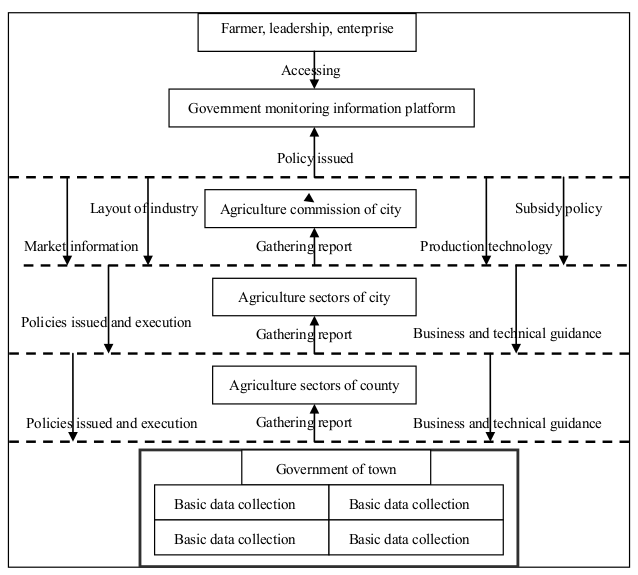
\includegraphics[scale=0.6,natwidth=\textwidth]{figures/designtools/businessrequirements.png}
 \centering
 \label{fig:fmishierarchy}
 \caption{Hierarchie von Datenquellen zu Entscheidungsträgern. \cite{jour:Wang2013}}.
\end{figure}

\subsection{Entwicklungen in der automatischen Auswertung}
Die Möglichkeit LCA in der Landwirtschaft einzusetzen wird in \textit{Streamlining life cycle inventory data generation in agriculture using traceability data and information and communication technologies – part I: concepts and technical basis} beleuchtet. Zu Beginn des Papers gehen die Autoren auf Probleme herkömmlicher LCAs ein:\cite{jour:Bellon-Maurel2014}
\begin{itemize}
	\item LCA als begleitende Maßnahme ist teuer da die Ermittlung der relevanten Daten aufwändig ist. Dementsprechend können nur große Betrieb LCA durchführen.
	\item Die herkömmlichen Messmöglichkeiten ermöglichen nur eine zeitverzögerte Reaktion die im Umfeld der Landwirtschaft zu Ausfällen führen können.
\end{itemize}

In ihrer Arbeit versuchen Bellon-Maurel, Short, Roux, Schulz und Peters den aktuellen Forschungsstand zusammen zu fassen und empfehlen den verstärkten Einsatz von ICTs um die LCI-Prozesse sie auf Kosten und Geschwindigkeit zu optimieren.\cite{jour:Bellon-Maurel2014}

Ein Faktor dessen Optimierungspotential durch Simulation erforscht wurde ist die maximale Lichteffizenz (\textit{maximum light efficency} $\varepsilon_{max}$. Wenquan, Yaozhang, Hao, Deyong und Haibo haben in \textit{Simulation of maximum light use efficiency for some typical vegetation types in China} gezeigt, dass der Fehlerintervall ihres Simulationsmodells klein genug ist um stabile und verlässliche Werte der Primärproduktion, kurz NPP, zu errechnen.  Damit kann bestimmt werden wo bestimmte Pflanzensorten angebaut werden können um den Ertrag zu maximieren. Die Basis für das Modell sind meterologische Daten, Vegetationskarten und vorhandene NPP-Daten.  \cite{jour:Zhu2006}

\subsection{Entwicklungen in Schwellenländern}

In der dritten Welt zeichnet sich durch die Verbreitung von Smartphones einer durch das Mobilfunknetz gestützte Schwarmintelligenz ab. Damit wird die Menge der Kontakte eines Bauers zu einem Orakel, dass zu den Themen Wetter, Ertrag und Best-Practices befragt werden können.\cite{jour:Razaque2013} Die Bedeutung der Übertragung von Informationen für den Ertrag und damit der Effizenz wird in \textit{Assessment of the Role of Mass Media in the Dissemination of Agricultural Technologies among Farmers in Kaduna North Local Government Area of Kaduna State, Nigeria} untersucht. Das Ergebnis war, dass sowohl Internet wie auch Fernsehen und Radio zur Verfügung stehen. Interessant dabei ist, dass in diesen Gebieten hauptsächlich Fernsehen- und Radioübertragung zur Verfügung stehen. Das Potential eine Schwarmintelligenz wie in \cite{jour:razaque2013} beschrieben aufzubauen ist vorhanden.\cite{jour:State2013}

Die Entwicklung der Abdeckung des Mobilfunknetzes in Indien und die gestarteten Projekte zur Steigerung des Ertrags mittels Mobilfunkprojekten wird in \textit{Use of Mobile Technologies for Empowering Small holder farmers in India} vorgestellt. Dabei werden Lösungen wie mKrishi vorgestellt, welches es den Bauern ermöglichen soll per Telephonanruf Fragen bezüglich der Landwirtschaftsarbeit in normaler Sprache zu stellen. \cite{article:Kokate2013}

\section{Expertensysteme in der Planung}
Ein Expertensystem ist ein KI-Programm, dass zwei Rollen annehmen kann.
\begin{itemize}
	\item \textit{Decision Maker}, als Entscheidungsfinder ermittelt das Expertensystem die qualitativ beste Lösung für ein gegebenes Problem. Z.B. die Behandlung eines Patienten mit definierten Symptomen oder die optimiale Bewässerung von Pflanzen.
	\item \textit{Oracle}, in diesem Fall dient das Expertensystem als Entscheidungshilfe in dem es gestellte Fragen beantwortet. 
\end{itemize}
Entscheidend für die Funktionalität des Expertensystems ist, dass ein Kausalmodell für die Problemdomäne gefunden wird, dieses zu einem quantitativen Entscheidungsmodell umgewandelt werden kann und daraus dann eine Entscheidung bzw. Antwort abgeleitet werden kann.\cite{book:Russell1995}

\begin{figure}[h]
 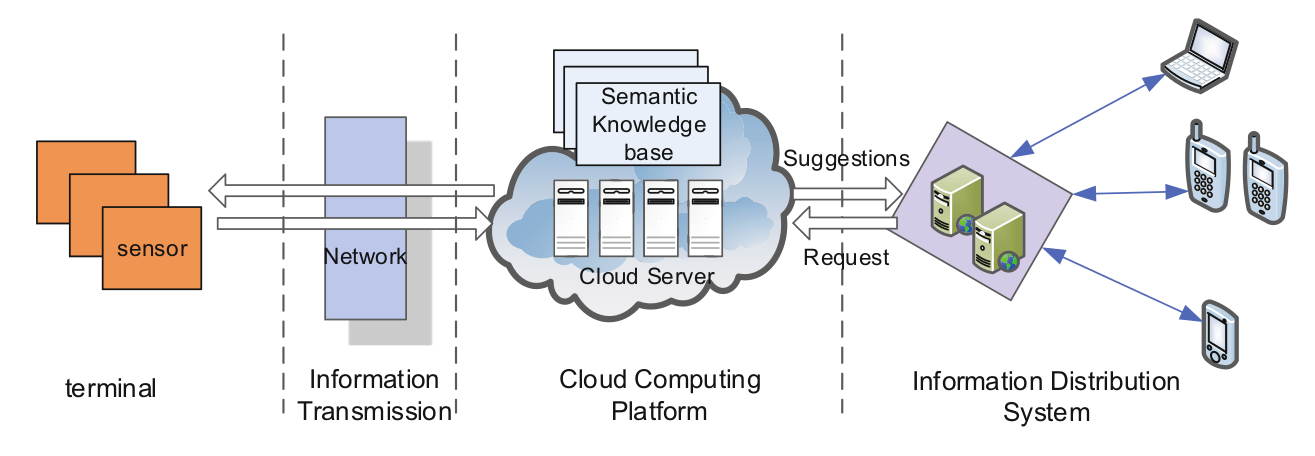
\includegraphics[scale=0.35,natwidth=\textwidth]{figures/designtools/cloud_iot_decisionmaker.png}
 \centering
 \label{fig:fmishierarchy}
 \caption{Architektur der Cloud-basierten Entscheidungshilfe.\cite{jour:Yuan2013}}.
\end{figure}

Lin, Nan, Li, Dongming, Bi und Chunguang stellen in \textit{Research on Development of Corn Production Decision} eine mögliche Architektur für ein System vor, dass bei der Planung und Pflege von Mais helfen soll. Dabei stellen sie folgende Best-Practices vor: 
\cite{jour:Lin2013}

\begin{itemize}
	\item Die Systemarchitektur und die Verwendung müssen als UML-Diagramme abgebildet werden. (Use-Case-Diagramme, Aktivitätsdiagramme, etc.)
	\item Die Datenbankstruktur muss als ER-Diagramm abgebildet werden.
	\item Die nötigen Objekte sollen mit der \textit{Object Definition Language}, kurz ODL, definiert werden.
	\item Die Verwendung der \textit{Framework Representation} um die Hierarchie und damit Kausalität von bestimmten Eigenschaften und Ereignissen abzubilden. (Z.B. ist ein Teil-Frame des Zustands von Gras dessen Halmzustand oder eine Erkrankung Teil des Disaster-Frames.)
\end{itemize}

Das in \textit{A new Expert System for greenness identification in agricultural images} vorgestellte Expertensystem dient dazu, die grüne Färbung der Blätter zu bestimmen. Dies kann z.B. dazu genutzt werden um die Wasserversorgung bedarfsorientiert zu gewährleisten.\cite{jour:Romeo2013}

Um die Entscheidungsfindung besser in puncto Effizienz und Geschwindigkeit zu machen wird in \textit{A Semantic Technology Supported Precision Agriculture System: A Case Study for Citrus Fertilizing} ein Cloud basiertes System vorgestellt. \cite{jour:Yuan2013}

Yuan, Zeng und Zhang stellen in ihrer Arbeit ein Expertensystem auf Basis eines Wissensbasierten System vor. Dabei werden Daten aus einem Sensornetzwerk als Ontologien abgebildet. Diese werden in der Cloud gespeichert. In der Cloud sitzt auch das Expertensystem, dass in der Lage ist Entscheidung zu treffen. Die Gesamtheit dieses Systems wird auch \textit{Semantic Technology} genannt.\cite{jour:Yuan2013}

Semantic Technology, kurz ST, bezeichnet dabei die Technologie die vorhandene Daten als  Ontologien aufbereiten um automatisiert Entscheidung ableiten zu können. Die in \textit{The Implementation of Layered Sensor Network Based on Semantic Technology} vorgestellte Architektur ST die ein Expertensystem und ein Sensornetzwerk verknüpft wird von Yuan, Zeng und Zhang wiederverwendet.\cite{jour:Liu2012}

\section{Planungswerkzeuge}

\subsection{Planungswerkzeuge für Freiluftunternehmen}
Im Gegensatz zu Glashäusern sind Felder der Umwelt schutzlos ausgeliefert. Das bedeutet, dass sich die Umweltfaktoren schnell ändern können und nicht alle Faktoren ausgeglichen werden können. (z.B. können Pflanzen nicht gegen Hagel geschützt werden.)

Den Einsatz von Ingenieurswerkzeugen um einen bestimmten Ertrag (z.B. Ernte, Kohle, etc.) zu produzieren werden \textit{Open Air Engineering}-Prozesse genannt. Diese Arbeiten zeichnen sich auch dadurch aus, dass im Betrieb eine Menge von verschiedenen Fahrzeugen und Arbeitern zusammen wirken müssen. (z.B. Mähdrescher, Traktoren um Pflügen, Traktoren um Wasserpumpen zu betreiben, etc.)

In \textit{PROSA and Delegate MAS for Open-Air Engineering Processes} stellen Valckenaers und Belle auf ein Planungskonzept für Open Air Engineering Prozesse vor. Die Basis ist eine Umsetzung der PROSA-Architektur um die im Prozess beteiligten Akteure als Agenten zu modellieren. Diese Agenten können dann in einer Simulation getestet werden um Probleme in der Ausführung erkennen zu können.\cite{conf:Valckenaers2011}

